\section{目的}

依講義 PDF 第 99--106 頁完成九項動態邏輯實驗：charge sharing、外加與寄生耦合、漏電、三種修復方式與 500 MHz 功耗比較。

\section{講義要求與對應測試}

\begin{center}
\small
\setlength{\tabcolsep}{4pt}
\begin{tabular}{p{.42\linewidth}p{.29\linewidth}p{.18\linewidth}}
\toprule
要求 & 網表編號與條件 & 狀態 \\
\midrule
步驟 1：NAND charge sharing & 01; A rises, B=0 & 已量測 \\
步驟 2--4：CC 掃描、翻轉、移至輸出 & 02; 5--50 fF & 門檻範圍已觀察 \\
步驟 5--6：NAND 上/下管寄生耦合 & 03; intrinsic coupling & 已量測 \\
步驟 7：長評估期漏電 & 04; 20 us, 25/115 C & 已量測 \\
步驟 8：常開/回授 keeper & 04/05/06; 500 MHz & 保持、sharing、功耗 \\
步驟 9：內部節點預充 & 04/05 & sharing 與漏電分辨 \\
\bottomrule
\end{tabular}
\end{center}

\section{電路與推導}

動態 NAND 在低 clock 預充，高 clock 評估。為使實驗可重現，輸出與串接內部節點各加入 5 fF，並保留 MOS 本身寄生。忽略損失的兩電容均分估算為 $V_f=(C_YV_{Y0}+C_XV_{X0})/(C_Y+C_X)$，但真實開關會受門檻、body effect、初始電位與 feedthrough 限制，不能要求模擬精確等於理想均分值。

外部 aggressor 的快速電壓變化近似產生 $\Delta V_Y\simeq C_C\Delta V_A/(C_Y+C_C)$。驅動中 inverter 輸出有低阻回復路徑，浮接動態節點則可能保留錯誤電荷。keeper 使用 $W/L=0.3/2\,\mu\mathrm m$ 的弱 PMOS；內部預充 PMOS 為 $0.6/0.25\,\mu\mathrm m$。

\section{模擬設定與判讀方式}

以提供的加密 MOS 模型、1.0 V 供應、25\,$^\circ$C 為基準。1.0 V 是教學測試條件，並非已核實的額定電壓；沒有把本次結果當作講義原製程或原供應電壓的重現。除網表另註，$W_n/W_p/L=0.6/1.8/0.25\,\mu\mathrm m$，Bulk 接對應電源軌，輸出負載為 5 fF。傳輸閘與弱回授器件的例外尺寸均在網表明列。

使用 PrimeSim HSPICE S-2021.09 win64、\texttt{RUNLVL=6}、\texttt{ACCURATE} 及 \texttt{WARNLIMIT=100}。每份網表的主分析與 \texttt{.alter} 均完成，沒有 error 或 failed measurement；但模擬器仍回報加密區塊的警告被隱藏，因此不能宣稱模型無警告或警告無害。\texttt{.tran} 的列印間隔不是固定積分步長；求解器使用自適應步長。本次沒有把有限的掃描範圍當作完整製程認證。

除非另註，功能診斷以低電位 $V\leq0.2$ V、高電位 $V\geq0.8$ V 判定；這是本報告公開採用的判讀規則，不是講義給定的數值門檻，也不是已萃取的接收器雜訊容限。取樣正確不能排除取樣間毛刺。所有圖均由實際輸出資料重繪；\texttt{results/} 保存逐案例波形、量測與衍生比較 CSV。

公開網表不含模型載入路徑；模擬時在本機副本加入模型設定，模型本體不在交付資料內。網表檔名的前兩位數對應下表編號，各檔可獨立執行。

\section{結果}

未接輸出 inverter 的基本 sharing 案例中，Y 從 1.172805 V 降到 0.701010 V，下降 0.471795 V；內部 X 為 0.622395 V。起始超過 1 V 來自 clock feedthrough，並非把供應電壓提高。比較修復方式時另用完全匹配的 inverter 負載，因此那組的原始下降量不同，不能與此基準混算。

\begin{figure}[htbp]
\centering
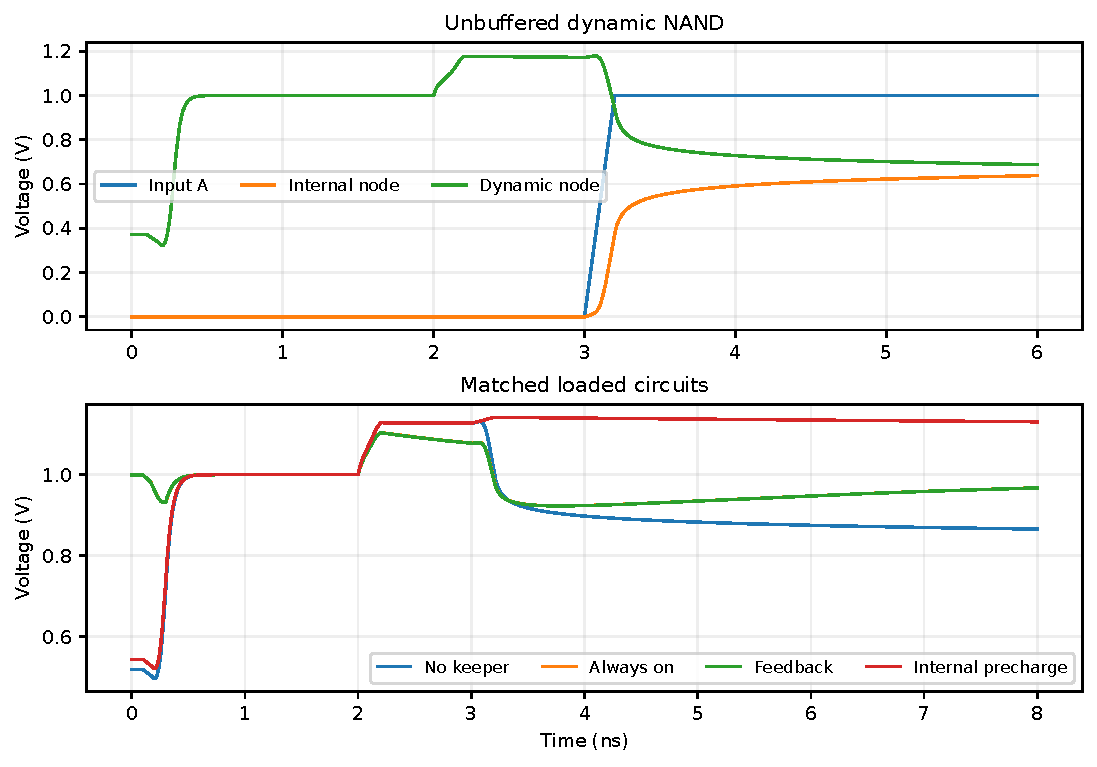
\includegraphics[width=.96\linewidth]{figures/charge_sharing.pdf}
\caption{基本 sharing 與同負載的三種修復比較。}
\end{figure}

\begin{center}
\small
\setlength{\tabcolsep}{4pt}
\begin{tabular}{lrrr}
\toprule
耦合 (fF) & 動態 Y (V) & inverter 輸出 (V) & 直接耦合輸出最低 (V) \\
\midrule
5 & 0.8277 & 0.0000 & -0.2632 \\
10 & 0.6555 & 0.0026 & -0.4427 \\
15 & 0.5511 & 0.0221 & -0.5547 \\
20 & 0.4845 & 0.2850 & -0.6161 \\
30 & 0.4027 & 0.9760 & -0.6562 \\
50 & 0.2859 & 0.9985 & -0.6843 \\
\bottomrule
\end{tabular}
\end{center}

CC=20 fF 時後級輸出為 0.284995 V，已落入本報告保守的不確定區；30 fF 時為 0.976020 V，形成明確錯誤高。以 0.5 V 作接收器判讀，轉換落在 20--30 fF 間。相同 30 fF 直接耦合 inverter 輸出會短暫降至 -0.656 V，但於 6 ns 回到約 0 V。這只是該測試窗的恢復，並非尖峰對任何接收器都無害。

\begin{figure}[htbp]
\centering
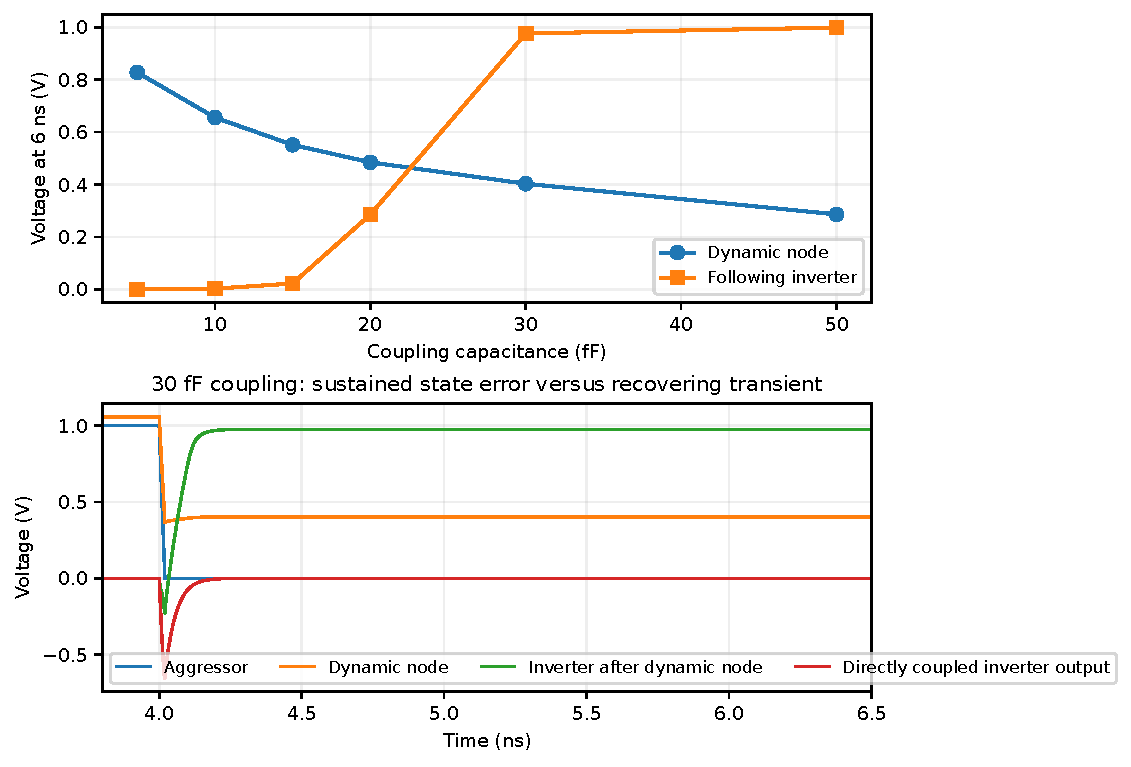
\includegraphics[width=.96\linewidth]{figures/coupling.pdf}
\caption{CC 掃描與 30 fF 代表波形；區分持續錯誤與可回復尖峰。}
\end{figure}

\begin{center}
\small
\setlength{\tabcolsep}{4pt}
\begin{tabular}{lrrr}
\toprule
NAND gate 位置 & 耦合前 (V) & 耦合後 (V) & 下降 (V) \\
\midrule
upper & 1.13912 & 0.94524 & 0.19388 \\
lower & 1.12564 & 1.07639 & 0.04925 \\
\bottomrule
\end{tabular}
\end{center}

不加入外部 CC、只保留器件寄生時，上 NMOS gate 耦合到 Y 的下降為 0.193876 V，下 NMOS 為 0.049251 V。這支持 gate/source/drain 位置與中間節點屏蔽會改變耦合，不是所有相同邏輯輸入 pin 都有相同類比敏感度。

\begin{figure}[htbp]
\centering
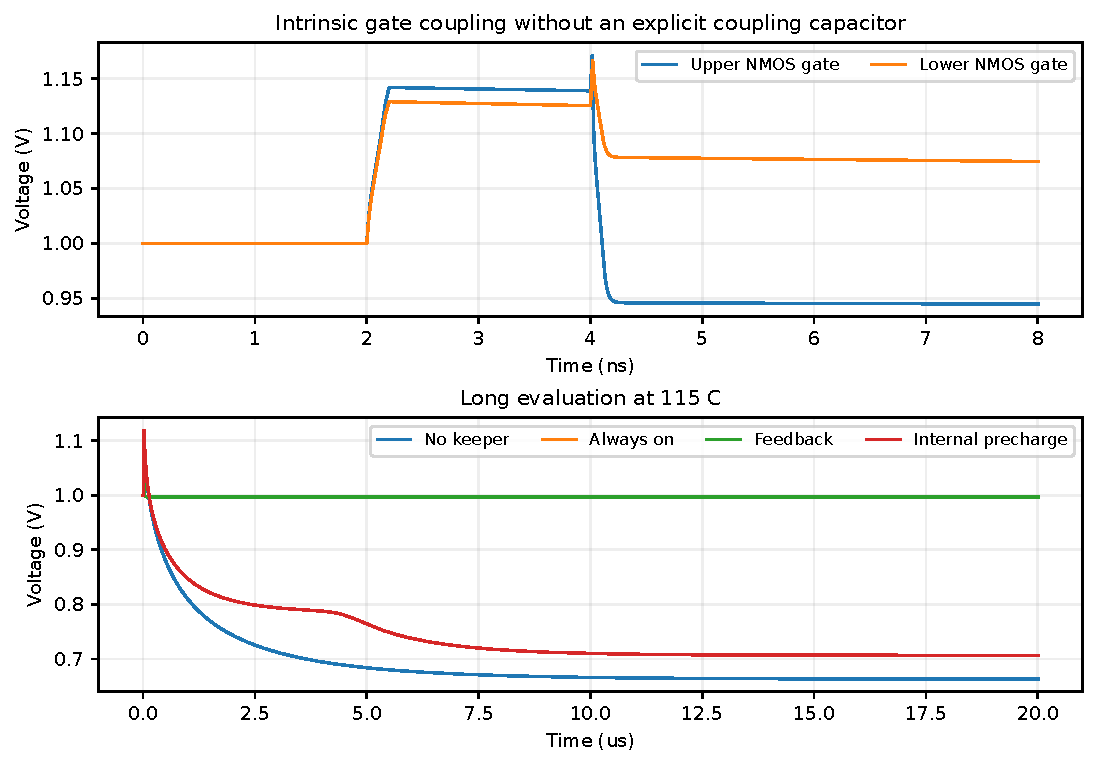
\includegraphics[width=.96\linewidth]{figures/coupling_and_retention.pdf}
\caption{上圖比較器件寄生耦合；下圖比較 115 C、20 us 保持。}
\end{figure}

\begin{center}
\small
\setlength{\tabcolsep}{4pt}
\begin{tabular}{lrrr}
\toprule
方式 & sharing 下降 (V) & 25 C 最終 (V) & 115 C 最終 (V) \\
\midrule
None & 0.24463 & 0.53783 & 0.66294 \\
Always on & 0.14851 & 0.99896 & 0.99702 \\
Feedback & 0.14830 & 0.99896 & 0.99702 \\
Internal precharge & -0.01016 & 0.58577 & 0.70663 \\
\bottomrule
\end{tabular}
\end{center}

常開與回授 keeper 將長保持電位維持在約 0.997--0.999 V；內部預充有效抑制 sharing，但並未提供評估期持續補電。未修復節點在 115 C 的最終值反而高於 25 C，顯示此模型與偏壓下淨電流由多個路徑決定；不可把結果改寫成溫度越高必然掉得越快。20 us 內此案例沒有觀察到完整 inverter 邏輯翻轉。

\begin{center}
\small
\setlength{\tabcolsep}{4pt}
\begin{tabular}{lrrrr}
\toprule
頻率 (MHz) & 常開功率 (uW) & 回授功率 (uW) & 常開評估 (uA) & 回授評估 (uA) \\
\midrule
500 & 16.1263 & 16.5449 & 9.9347 & 8.2381 \\
50 & 2.4854 & 1.6582 & 1.8482 & 0.6664 \\
\bottomrule
\end{tabular}
\end{center}

\begin{figure}[htbp]
\centering
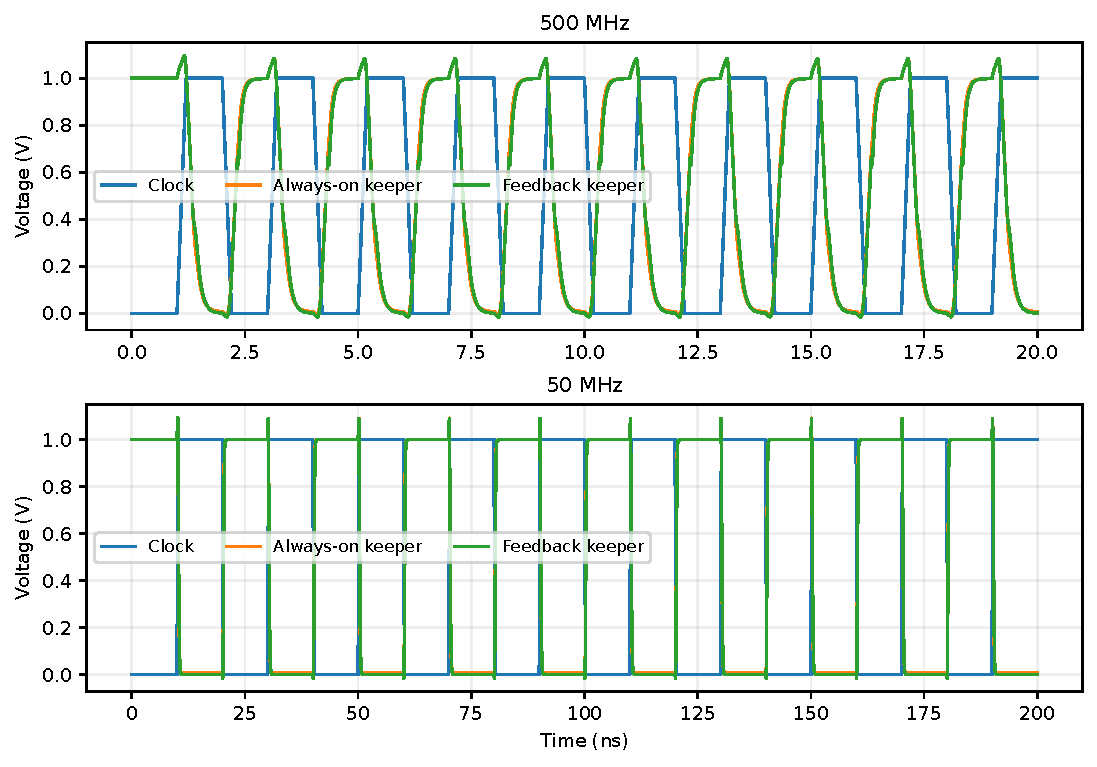
\includegraphics[width=.96\linewidth]{figures/keeper_power.pdf}
\caption{保留講義 500 MHz，另加 50 MHz 作較充分建立的對照。}
\end{figure}

\section{討論、差異與尚未證實的範圍}

500 MHz 時回授平均功率 16.5449\,$\mu$W 略高於常開 16.1263\,$\mu$W，不能強行宣稱回授必然較省電。其評估期電流較低，但整週期平均還包含動態充放電、延遲及切換競爭；50 MHz 時回授平均功率才降至 1.6582\,$\mu$W，低於常開 2.4854\,$\mu$W。功率平均取 $2T$--$10T$，評估電流取 $8.7T$--$8.9T$。九項觀察均有對應測試，未把講義的定性解釋當作硬性數值 pass/fail。
